\documentclass[runningheads]{ola}
% The preceding line is only needed to identify funding in the first footnote. If that is unneeded, please comment it out.
\usepackage{tikz}
\usetikzlibrary{shapes, arrows, positioning, fit,backgrounds}

\usepackage{subcaption}
\usepackage{multicol}
\usepackage{multirow}
\usepackage{amsmath}
\usepackage{algorithm}
\usepackage{algpseudocode}
\usepackage[acronym, toc, xindy, ucmark]{glossaries}
\usepackage{amsfonts}
\usepackage{hyperref}
\usepackage{placeins}
\usepackage{blindtext}
\makeglossaries
\newacronym{llm}{LLM}{Large Language Model}

\newacronym{lhs}{LHS}{Latin Hypercube Sampling}
\newacronym{gp}{GP}{Gaussian Process}
\newacronym{soo}{SOO}{Simultaneous Optimistic Optimization}
\newacronym{bamsoo}{BaMSOO}{Bayesian Multi-scale Optimistic Optimization}
\newacronym{bo}{BO}{Bayesian Optimization}
\newacronym{smbo}{SMBO}{Surrogate Model-Based Optimization}
\newacronym{mcts}{MCTS}{Monte Carlo Tree Search}
\newacronym{ucb}{$\mathcal {UCB}$}{Upper Confidence Bound}
\newacronym{lcb}{LCB}{Lower Confidence Bound}
\newacronym{hpc}{HPC}{High Performance Computing}
\newacronym{nlp}{NLP}{Natural Language Processing}
\newacronym{gpu}{GPU}{Graphic Processor Unit}
\newacronym{sota}{SOTA}{State-of-the-art}
\newacronym{peft}{PEFT}{Parameter Efficient Fine-Tuning}
\newacronym{lora}{LoRA}{Low-Rank Adaptation}
\newacronym{pbo}{PBO}{Partition Based Optimization}
\newacronym{dnn}{DNN}{Deep Neural Networks}

\newglossaryentry{hs}
{
    name=hellaswag,
    description={empty}
}

\newglossaryentry{hp}{
name = hyperparameter,
plural = hyperparameters,
description = {empty}
}
\newacronym{hpo}{HPO}{\Gls{hp} Optimization}
\newacronym{automl}{autoML}{Automated Machine Learning}
\newacronym{autodnn}{autoDNN}{Automated Deep Neural Networks}
\newacronym{bogp}{BO-GP}{Bayesian Optimization based on Gaussian Process}
\newacronym{mvop}{MVOP}{Mixed-Variables Optimization Problem}
\newacronym{mha}{MHA}{Multi-Head Attention}
\begin{document}

\pagestyle{headings}

\mainmatter

\title{Bayesian and Partition-Based Optimization for Hyperparameter Optimization of LLM Fine-Tuning}
% Title
\titlerunning{\acrshort{bo} and \acrshort{pbo} for \acrshort{hpo} of LLM Fine-Tuning}


\author{N. Davouse and E-G. Talbi}

% Authors for the top of the even pages
\authorrunning{N. Davouse and E-G. Talbi}

\institute{Univ. Lille, CNRS, Inria, Centrale Lille, UMR 9189 CRIStAL, F-59000 Lille, France \\
\email{nathan.davouse@inria.fr and el-ghazali.talbi@univ-lille.fr}\\
}

\maketitle

\begin{abstract}
\acrfull{llm}s have revolutionized natural language processing (NLP) by achieving state-of-the-art performance across diverse tasks. However, fine-tuning these models for domain-specific applications is significantly constrained by the computational costs associated with their training. In this paper, we propose two complementary approaches to address the \acrfull{hpo} challenge in LLM fine-tuning: \acrfull{bogp} and \acrfull{pbo}. On one hand, \acrshort{bo} efficiently exploits historical knowledge to achieve optimal results within a limited number of evaluations, but its inherently sequential nature poses scalability challenges. On the other hand, \acrshort{pbo} enables massive parallelization, making it more scalable but requiring significantly more evaluations to converge. To leverage their complementary strengths for optimizing expensive objective functions, we investigate these methods and propose a hybrid \acrshort{bo}-\acrshort{pbo} algorithm. This work represents a foundational step toward harnessing the potential of parallel \acrlong{bo}-based algorithms for solving expensive optimization problems in exascale computing environments.
\end{abstract}


\section{Introduction}
\label{sec:intro}

With the advent of transformer architecture\cite{vaswani_attention_2017}, coupled with significant advancements in the field of \acrfull{hpc}, \acrfull{llm}s have demonstrated exceptional abilities in language understanding and text generation, firmly establishing themselves as the \acrfull{sota} in \acrfull{nlp}. Models such as GPT-4 \cite{openai_gpt-4_2024} and LLaMA 3 \cite{grattafiori_llama_2024} have rapidly penetrated the personal and professional domains, transforming workflows in academic, industrial and everyday applications.

Despite their success, the computational and data requirements for training LLMs from scratch make this approach impractical for most users. Fine-tuning has emerged as a critical paradigm, adapting pre-trained models to specialized tasks using smaller domain-specific datasets. Although fine-tuning reduces costs compared to full training, it remains resource intensive, particularly for large-scale models. To address this, \acrfull{peft} methods \cite{han_parameter-efficient_2024}, such as Low-Rank Adaptation (LoRA) \cite{hu_lora_2021}, have become prevalent. LoRA and its derivatives (e.g., QLoRA \cite{dettmers_qlora_2023}, LoRA + \cite{hayou_lora_2024}) reduce computational overhead by using reparameterized weight matrices, where large weight matrices are approximated with lower-rank decompositions. This approach enables fine-tuning even on limited-hardware setups.

Even with advancements in \acrshort{peft}, a significant barrier persists: selecting optimal hyperparameters. Unlike model parameters, which are learned during training, hyperparameters must be manually specified and profoundly influence model performance. For \acrshort{lora}-based fine-tuning, hyperparameters such as rank and scaling factors are critical\cite{valipour_dylora_2023}, along with classical parameters such as learning rate and weight decay.

\acrfull{hpo} is a well-studied problem \cite{bischl_hyperparameter_2021,bergstra_algorithms_2011,feurer_hyperparameter_2019} in \acrfull{autodnn} design \cite{talbi_automated_2021}. However, \acrshort{hpo} for LLM fine-tuning presents unique challenges due to the prohibitive cost of evaluating the objective function. Each evaluation entails computationally expensive training or fine-tuning process, often requiring hours to days on high-performance hardware. These constraints necessitate the adoption of highly efficient optimization techniques.

\acrfull{bo} \cite{shahriari_taking_2016} is a widely recognized approach for tackling expensive black-box optimization problems. Its ability to model the search space using a surrogate function allows it to minimize costly evaluations. However, \acrshort{bo} is by nature sequential, limiting the use of \acrshort{hpc} cluster, or exascale computer.
In contrast, \acrfull{pbo} methods \cite{nakib_deterministic_2017,munos_optimistic_2011}, which divide the search space into sub-regions, enable parallel evaluations but typically require more function calls to converge. The complementarity of theses methods made way for hybrid algorithms, using surrogate to enhance \acrshort{pbo} algorithms.

In this work, we present the \acrshort{hpo} problem for \acrshort{llm} fine-tuning, to address it with \acrlong{bo} and \acrlong{pbo} methods. By comparing theses methods, and trying the hybridization, we aim to open the way for parallel Bayesian algorithm for optimization of very expensive objective function with exascale computing.

\newcommand{\Dtrain}{\mathcal{D}_{train}}
\newcommand{\Dval}{\mathcal{D}_{val}}
\newcommand{\model}{\mathcal{M}}

\section{Problem definition}
\label{sec:pbm}

\acrfull{hpo} of \acrshort{llm} Fine-Tuning is a very recent problem in literature, with a first review on article \cite{LiuEmpirical2021}, but \acrshort{hpo} for \acrfull{dnn} is a known field with the \acrshort{automl} community. For further reading, a taxonomy of \acrshort{autodnn} can be found with article \cite{talbi_automated_2021}. 

This problem can be classified as a black-box objective function optimization, i.e. the objective function cannot be formulated analytically and can't be derived. This characteristic constrain the sets of methods to be used directly. Following article \cite{talbi_metaheuristics_2024} notation, this problem is also a \acrfull{mvop}, w.r.t. the set of values possible for each \gls{hp}. The last key aspect of this optimization problem is the cost of evaluating a solution, it can take dozens of minutes to hours, restraining the number of possible evaluations.

Given a model $\mathcal M$, a training dataset $\Dtrain$, a validation dataset $\Dval$ and a set of hyperparameters $\eta$, the black-box function can be expressed as $  \mathcal F(\eta, m,\mathcal{D}_{train},\mathcal{D}_{val})$. This function includes the training of the model, and also the evaluation using $\Dval$, and allow to link hyperparameters to training and to evaluation. In this work, the optimization is solely single objective, so the result of the function $\mathcal F$ is in $\mathbb{R}$.

Given this function, the optimization problem can be expressed as equation \ref{eq:opt_def}, where $\mathcal{H}$ is the search space of hyperparameters. The aim of this problem is to find one value being the maximum of the function $\mathcal F(.\space,\space.\space, \space .\space, \space .)$. 


\begin{equation}
    \eta^* \in \arg\max_{\eta \in \mathcal{H}} \mathcal{F}(\eta,\model,\mathcal{D}_{train},\mathcal{D}_{val})
\label{eq:opt_def}
\end{equation}

%%%%%%%%%%%%%%%%%%%%%%%%%%%%%%%%%%%%% Search Space %%%%%%%%%%%%%%%%%%%%%%%%%%%%%%%%%%%
\subsection{Search Space}
\label{sec:search_space}

The search space is defined with the choice of hyperparameters, theirs bounds, theirs types and even theirs scales.  Well-defined search space is crucial for a correct application of \acrshort{hpo} : if the space is too high-dimensional, the \acrshort{hpo} algorithm will need too many shots to converge to a good solution, if it's too small, we are missing it's relevance. 

\begin{equation}
    \begin{split}
    W = W_0 + \Delta W = W_0 + \frac{\alpha}{r}(B.A) \\
    s.t. \quad W,W_0,\Delta W \in \mathbb{R}^{n*p},
    A \in \mathbb{R}^{r*p} \text{ and } B \in \mathbb{R}^{n*r}
    \end{split}
    \label{eq : lora}
\end{equation}

The search space is composed of 5 hyperparameters, from classical training hyperparameters to \acrshort{lora} specific ones. Equation \ref{eq : lora} summarize \acrshort{lora} application, w.r.t. it's \gls{hp}, with $W_0$ the weights of the pre-trained model and $W=\Delta W$ the additional gradients to add to obtain $W$ the weights of the fine-tuned model. A detailed presentation of hyperparameters is just below, but one can look at table \ref{tab:hyperparam_table} for a summary.
\begin{itemize}
    \item LoRA rank : the common rank of matrices $A$ and $B$, scaling the reduction in terms of number of parameters. It's an integer, and it's value range from 1 to 64 to deal with hardware constraints.
    \item LoRA scale ($\alpha$) : $\alpha$ is used to scale the values of $B*A$ when added to $W_0$. On this work, due to LitGPT framework, it's an integer, from 1 to 64.
    \item Learning rate : the learning rate is a classical \gls{hp} used in \acrshort{hpo}, weighting the gradient of each weight when doing back-propagation. It is often tuned in a logarithmic scale, to manage effectively the exploration. \Gls{hp} value is between $10^{-10}$ and $10^{-1}$.
    \item Dropout probability : based on article \cite{srivastava_dropout_2014}, dropout is a method used to prevent over-fitting, by randomly fixing cells/layers to zeroes during one iteration. Being a probability, it's bounds by 0 and 1.
    \item Weight decay : weight decay is used to improve generalization capacity, as proved in article \cite{krogh_simple_1991}, by reducing the weights at each iterations by a small value, to force the model to use new inputs. Typically, the parameter for weight decay is set on a logarithmic scale between $10^{-3}$ and $10^{-1}$.
\end{itemize}

\vspace*{-\baselineskip}
\begin{table}[h]
    \centering
    \begin{tabular}{|c|c|c|c|c|}
        \hline
        \multirow{2}{*}{\textbf{ \Gls{hp} }} & \multicolumn{2}{|c|}{\textbf{Optimization range}} &\multirow{2}{*}{\textbf{ Type }}& \multirow{2}{*}{\textbf{ Conversion }} \\
        \cline{2-3}
         & \textbf{ Lower Bound } & \textbf{ Upper Bound } &  \\
        \hline
        \textbf{Learning Rate} & $-10$ & $-1$ & log. & $f(x) = 10^{x}$ \\
        \hline
        \textbf{LoRA Rank} & 2 & 32 &int. &$f(x) = \text{round}(x)$ \\
        \hline
        \textbf{LoRA scale ($\alpha$)} & 16 & 64 & int. &$f(x) = \text{round}(x)$ \\
        \hline
        \textbf{LoRA Dropout} & 0 & 0.5 & cont.& $f(x) = x$ \\
        \hline
        \textbf{Weight Decay} & $-3$ & $-1$ &log.& $f(x) = 10^{x}$  \\
        \hline
    \end{tabular}
    \caption{Summary of Hyperparameter Search Space}
    \label{tab:hyperparam_table}
\end{table}\vspace*{-\baselineskip}

For the 2 integers variables (LoRA rank and LoRA scale), to adapt to continuous optimization algorithms, the relax and round methods will be applied. It mean that the integers constraints is relaxed when generating a solution, and is rounded when evaluating a solution. Others methods like computing with lower and upper discrete value can be used, but this one was kept for simplicity and computation costs.
For the 2 variables with logarithmic scale (learning rate and weight decay), to explore with consistency the search space, the optimization algorithm will be bound between the exponential values of the bounds, and a logarithm will be applied when evaluating a solution.


%%%%%%%%%%%%%%%%%%%%%%%%%%%%%%%%%%%%% Objective Function %%%%%%%%%%%%%%%%%%%%%%%%%%%%%%%%%%%
\subsection{Objective Function}
\label{sec:obj_fun}
Classically with DNN, the function to optimize might be the loss , sometimes normalized like Cross-entropy Loss or the accuracy. To avoid data leakage, the function is computed over a validation dataset, and even a testing dataset, different from the training one. For LLM, the datasets are a lot more diverse than for images classification, and the loss is biased to value the performance of a LLM, since it take all probabilities inside the function. 

A second option to evaluate LLM fine-tuning is to use the accuracy over standard benchmarks, using multiple-questions choices to process an efficient evaluation of the performance of the LLM. Article like \cite{wei_finetuned_2022} explain that fine-tuned model have better generalization performance, so it's relevant to evaluate on a different dataset than the training, even if the layout of the inputs change. State-of-the-art example for fine-tune model are HELLASWAG\cite{zellers_hellaswag_2019} or MMLU\cite{hendryckstest2021,hendrycks2021ethics}. In this papers, the function to maximize with the HPO is the accuracy on the Hellaswag datasets.


%%%%%%%%%%%%%%%%%%%%%%%%%%%%%%%%%%%%% Related Works %%%%%%%%%%%%%%%%%%%%%%%%%%%%%%%%%%%

\subsection{Related work}
\label{sec:related}
To locate this work on a global fields, this section aims to review relevant problematic and contributions close to this paper. 

\begin{itemize}
    \item AutoDNN : the global autoDNN fields has been thoroughly explored last years. Article \cite{talbi_automated_2021} make a review and a taxonomy of this global fields. HPO applied to LLM fine-tuning differs from this especially by the cost of evaluation and the evaluation of the model. Methods or specific problem of \acrshort{autodnn} are now infeasible with LLM due to the costs. Specific methods are then needed.
    \item LLM applied to EA : when looking at interaction between LLM and EA, a lot of articles \cite{liu_large_2024,cai_exploring_2024,brahmachary_large_2024} are using LLM to enhance or popularize EA and optimization algorithms. This approach isn't relevant to our contribution, since our contribution focus on our optimization expertise. 
    \item Prompt optimization : when linking optimization and LLM, some papers \cite{diao_black-box_2023,xu_gps_2022} aims to optimize the prompt, and work with the entire LLM as a generating blackbox, without thinking about the architecture or the weights. This approach have limited effects on LLM, since the performance are still bound by model training, and they replace the end users for chat-bot deployment. 
    \item HPO applied to generation \gls{hp} : some \glspl{hp} like the \textit{temperature} are only used when \acrshort{llm} are generating tokens. Some are working of theses hyperparameters, to avoid training costs of working directly with the fine-tuning hyperparameters.  
\end{itemize}




\section{Design and Implementation}
\label{sec:methodo}
In this work, two approaches are considered to performs \acrfull{hpo} : \acrfull{bogp} and \acrfull{pbo} algorithms like \acrfull{soo}\cite{munos_optimistic_2011}. To extract the best of these two approaches, an hybrid approach will also be presented.

Figure \ref{fig:workflow} describe the global workflow of \acrfull{hpo}, to link with following sections aiming to describe sections of the workflow. 

\begin{figure}
    \centering
    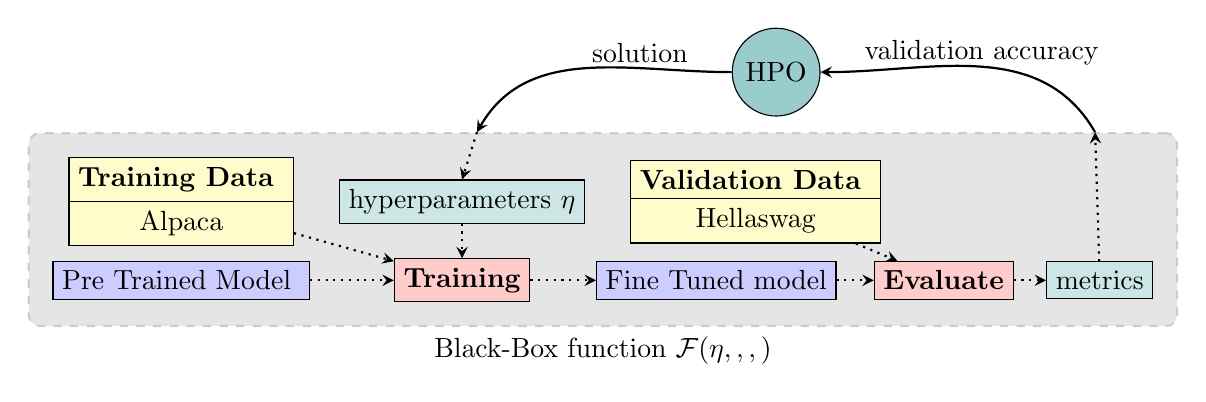
\begin{tikzpicture}
    \tikzstyle{data}=[rectangle split, rectangle split parts = 2,draw,text centered, fill=yellow!20]
    \tikzstyle{model} = [rectangle, draw, text centered, fill = blue!20]
    \tikzstyle{function} = [rectangle, draw, text centered, fill = red!20, font = \bfseries]
    \tikzstyle{metrics} = [rectangle, text centered, draw, fill=teal!20]
    
\tikzstyle{dot_arrow} = [thick,dotted,->,>=stealth]

\node (train_data) [data]
    {
        \textbf{Training Data $\Dtrain$}
        \nodepart{second} Alpaca};  

\node (PT_model)[model, below of = train_data]{Pre Trained Model $\model$};

\node (training) [function, right of = PT_model, anchor = west, xshift = 1.7cm]{Training};

\node (hp) [metrics, above of = training]{hyperparameters $\eta$};

\node (FT_model) [model, right of = training, anchor = west, xshift = 0.7cm]{Fine Tuned model};

\node (val_data) [data, above of = FT_model, xshift = 0.5cm]
    {
        \textbf{Validation Data $\Dval$}
        \nodepart{second} Hellaswag}; 
        
\node (evaluate) [function, right of = FT_model, anchor = west, xshift = 1cm]{Evaluate};

\node (metrics) [metrics, right of = evaluate, anchor = west, xshift = 0.3cm]{metrics};


\begin{scope}[on background layer]
    \node(bbfunction)[draw, thick,fill=black!10,draw=black!20, dashed, rounded corners, fit=(train_data) (PT_model) (training) (FT_model)(val_data)(evaluate)(metrics), inner sep=0.3cm, label=below:{Black-Box function $\mathcal F (\eta, \model, \Dtrain,\Dval)$ }] {};
\end{scope}

\draw [dot_arrow] (train_data) -- (training);
\draw [dot_arrow] (PT_model) -- (training);
\draw [dot_arrow] (hp) -- (training);
\draw [dot_arrow] ([xshift = -1.6cm]bbfunction.north) -- (hp.north);
\draw [dot_arrow] (training) -- (FT_model);
\draw [dot_arrow] (val_data) -- (evaluate);
\draw [dot_arrow] (FT_model) -- (evaluate);
\draw [dot_arrow] (evaluate) -- (metrics);
\draw [dot_arrow] (metrics) -- ([xshift = 6.25cm]bbfunction.north);

\node (hpo) [circle, above of = bbfunction, yshift = 1cm,xshift=2.2cm, draw, fill = teal!40]{HPO};
\node [left of = hpo, yshift = 0.25cm, anchor = east]{solution};
\node [right of = hpo, yshift = 0.25cm,anchor = west]{validation accuracy};

%\draw [thick,->,>=stealth]    ([xshift = 6.25cm]bbfunction.north) to[out=90,in=-5] (hpo.east);
\draw [thick,<-,>=stealth]     (hpo.east)to[out=0,in=120] ([xshift = 6.25cm]bbfunction.north);
\draw [thick,->,>=stealth]     (hpo.west) to[out=180,in=60] ([xshift = -1.6cm]bbfunction.north);




\end{tikzpicture}
    \caption{ \acrshort{hpo} workflow}
    \label{fig:workflow}
\end{figure}\vspace*{-\baselineskip}

The workflow is budget-based, meaning all algorithms will be compared with the same number of evaluations, i.e., the budget. This approach is effective because it ensures a fair comparison by focusing on the evaluation cost, which is the primary bottleneck in optimization scenarios, rather than computational overhead, which is negligible in this context. The computing time of the algorithm is negligible in front of evaluation time, making the number of evaluation a relevant budget metric. 

%%%%%%%%%%%%%%%%%%%%%%%%%%%%%%%%%%% LLM %%%%%%%%%%%%%%%%%
\subsection{Fine-tune and evaluate LLM}
\label{sec:llm}
\acrshort{hpo} is a problem defined by a specific black-box function, and must adequate with the characteristic of this objective function. As said in section \ref{sec:pbm}, in this work, the function can be defined as an expensive, mixed-variables, noisy black-box function. This part aims to present this function, allowing to reproduce it. 

The backbone model is LlaMa 3.2-1B \cite{grattafiori_llama_2024}, a model of the Llama 3 family of model. Llama 3 models were released by Meta AI in the second part of 2024 (from July to December), as open-source (topology and weights) decoder-only models achieving state-of-the-art performance. Among Llama 3 models, Llama 3.2 release propose lightweight models (from 1B to 3B weights, excluding vision models), enabling reproduction of the experiments. 

The fine-tuning is performed using AdamW \cite{loshchilov_decoupled_2019} optimizer, along \acrshort{lora} methods to keep efficient fine-tuning. To achieve performance comparable with full fine-tuning, \acrshort{lora} is used on keys, queries, values and attention head output weight matrices, enabling the training of whole \acrfull{mha} layers. 

Then, the training data $\Dtrain$ is the \textit{Alpaca} dataset, published after the \textit{Standford Alpaca Project}. It's composed of 52k lines of IA generated and cleaned inputs, aiming to improve the behavior of a LLM. This dataset is widely used \cite{dettmers_qlora_2023,chung_scaling_2024,zhou_lima_2023} for fine-tuning, guiding our choice for a standard configuration. 

For evaluation, Hellaswag \cite{zellers_hellaswag_2019} dataset was used as $\Dval$, with accuracy as the metrics to optimize with \acrshort{hpo}. It's a 40k lines datasets released in 2019 as a challenge datasets, with a random performance of 25 \% . All models are also evaluated on MMLU \cite{hendryckstest2021} as a testing dataset, to observe \acrshort{hpo} over-fitting. 

In terms of framework, all this part is done using LitGPT \cite{the_lightning_ai_team_litgpt_2023}, a framework develop by Lightning AI team, based on Pytorch  \cite{ansel_pytorch_2024} environment. This framework is thought for a command line interface utilization, and will be kept as it is in this work. Behind this framework, it's PyTorch for training the model, Huggingface for loadings model and datasets, and lm\_eval library for managing evaluation.

%%%%%%%%%%%%%%%%%%%%%%%%%%%%%%%% BO GP %%%%%%%%%%%%%%
\subsection{\acrfull{bo} : \acrfull{gp} based optimization}
\label{sec:bo}

Bayesian Optimization is often defined as a "sequential model-based approach to solving problem" \cite{shahriari_taking_2016}. A surrogate model is used to build a posterior considering a prior knowledge formed on known points. On this posterior, an acquisition function is computed to act as the surrogate function for the function to optimize. Many surrogate models can be used like regression tree \cite{ammari_linear_2023} or \acrfull{gp} \cite{rajaram_empirical_2021}. For further details about \acrshort{bo}, one can read review \cite{shahriari_taking_2016}.

On this work, a focus is done on \acrshort{gp} for the \acrshort{bo} surrogate. \acrshort{gp} use the kernel trick to build a bayesian nonparametric regression model. It use a mean vector $m_i$ and a covariance matrix $K_{i,j}$ to define the prior function as equation \ref{eq:prior_gp}. 

\begin{equation}
    \text{f} | X \sim  \mathcal N (m,K)
    \label{eq:prior_gp}
\end{equation}

\begin{algorithm}[h]
\caption{\acrshort{bogp}}
\label{algo:bo}
\begin{algorithmic}[1]
\Require 
    $\Omega$,$f$,$K_D$,$\mathcal{O}$,$f_{\text{acq}}$,$n_{init} $,$n_{opt}$
        
\For{$i = 1$ \textbf{to} $n_{init}$} \Comment{Initiate with Latin Hypercube Sampling}
    \State $\lambda' \gets LHS(\Omega,\mathcal{D},n_{init})$ \Comment{Sample one point}
    \State $\mathcal{D} \gets \mathcal{D} \cup \{(\lambda', f(\lambda'))\}$ \Comment{Add solution and evaluation to set of data}
\EndFor 
\For{$i = 1$ \textbf{to} $n_{opt}$} \Comment{Optimization loop}
    \State $K_D,\mu_D \gets \text{Fit}(\text{GP}(K_D,\mu_D), \mathcal{D})$ 
    \State $\lambda' \gets \text{Optimize}(f_{\text{acq}}(K_D), \mathcal{O})$ \Comment{Generate new point}
    \State $\mathcal{D} \gets \mathcal{D} \cup \{(\lambda', f(\lambda'))\}$ \Comment{Evaluate new point}
\EndFor
\State \Return best of $\{(\lambda^*, f(\lambda^*)) \in \mathcal{D}\}$
\end{algorithmic}
\end{algorithm}

Algorithm \ref{algo:bo} offer an overview of the BO process. To ease the first build of the surrogate, it's crucial, as proven in article \cite{wilson_efficiently_2020}, to sample efficiently the search space. This sampling provides information for the Gaussian Process to estimate the function. Like article \cite{borisut_adaptive_2023}, \acrfull{lhs} is used as a sampling method, for a defined budget called $n\_init$. 

After this preliminary phase, a second phase is done with loop containing the update of the Gaussian Process, the optimization of the acquisition function to obtain a new points to evaluate and the evaluation. After the evaluation of the point, the point is added to the history $\mathcal D$ and so on. The loop end based on a budget $n_{opt}$, with the budget $n_{max}=n_{init}+n_{opt}$ 

For this algorithm, the first requirements is the search space, and the objective function already described in \ref{sec:search_space} and \ref{sec:obj_fun} respectively. On the \acrshort{gp} part, we need to define a Kernel function $K_\mathcal D$, an acquisition function $f_{acq}$ and an Inner Optimizer $\mathcal O$. The acquisition function is logEI, more reliable than EI, based on article \cite{ament_unexpected_2024}. The kernel and the inner optimizer are the standard implementation of Botorch, introduced in the next paragraph, with a radial basis function kernel and multi-start optimization method. 

BoTorch \cite{balandat_botorch_2020} is a Bayesian Optimization library built on PyTorch, designed for efficient and scalable optimization of expensive black-box functions. Leveraging PyTorch's GPU acceleration and integration with GPyTorch \cite{gardner_gpytorch_2021} for Gaussian Processes, BoTorch enables advanced surrogate modeling and optimization. Botorch is used on this work for all tasks using \acrshort{gp}, including this part and section \ref{sec:bamsoo}


%%%%%%%%%%%%%%%%%%%% SOO %%%%%%%%%%%%%%%%%%%%%%%%%%
\subsection{\acrlong{pbo} : \acrfull{soo}}
\label{sec:soo}
In global optimization, a lot of methods are based on the partition of the search space \cite{nakib_deterministic_2017,jones_lipschitzian_1993,munos_optimistic_2011}. Theses approaches are mostly deterministic, and enhance intrinsic parallelization ability. For theses methods, the dimensionality of the problem is a key to choose the specific algorithm. With a dimensionality around 5, based on benchmarks at the end of article \cite{firmin_fractal-based_2022}, the \acrfull{soo} \cite{munos_optimistic_2011} algorithm seems a good way to start. 

\begin{algorithm}
\caption{SOO}
\label{algo:soo}
\begin{algorithmic}[1]
\Require $\Omega$,$f$,$K$,$n_{max}$ 

\State $x_{0,0} \gets center(\Omega)$,$f_{0,0} \gets    f(x_{0,0})$,$\mathcal T_1 = \{x_{0,0},f_{0,0},\Omega\}$ \Comment{Initiate the tree with the center of $\Omega$}

\State $n \gets 1$

\While{$n < n_{max}$}
    \State $\nu_{max} \gets - \infty$
    \For{$h=0 \textbf{ to } depth(\mathcal T_n)$}
        \State $j \gets \arg \max_{j \in \{j | (h,j) \in L_n\}} f(x_{h,j})$ \Comment{Select best open leaf for depth $h$}
        \If{$f_{h,j} > \nu_{max}$}
            \State $\Omega_{h+1,kj+1},\dots,\Omega_{h+1,kj+K} \gets section(\Omega_{h,j},K)$ \Comment{perform K-section of $\Omega_{h,j}$}
            \For{$i=1$ \textbf{to}$K$}
                \State $n \gets n+1$
                \State $x_{h+1,kj+i} \gets center(\Omega_{n})$
                \State  { \color{blue} $f_{h+1,kj+i} \gets    f(x_{h+1,kj+i})$ \Comment{evaluate the point, the scoring}}
                \State $\mathcal T_n \gets \{(x_{h+1,kj+i},f_{h+1,kj+i},\Omega_{n+1})\}$ \Comment{Add $\text{leaf}_{h+1,j+i}$ to tree $\mathcal T_n$}
            \EndFor  
            \State $\nu_{max} \gets f_{h,j}$
        \EndIf
    \EndFor
\EndWhile\\
\Return best of $x_{h,j},f(x_{h,j})$
\end{algorithmic}
\end{algorithm}

\acrshort{soo} is a tree-based space partitioning method for black-box optimization, inspired by \acrfull{mcts} methods. \acrshort{soo} is called optimistic since it assume the existence of $ l$ such that $f(x^*)-f(x) \leq l(x,x^*)$ where $x^*$ is the maximizer of $x$.The algorithm partition the space $\Omega$ by building a tree with smaller and smaller sub-space $\Omega_{h,j}$. The node $(h,j)$, node number $j$ of depth $h$, is scored at the center of his space. 

An expanded node have $K$ children, making the tree a $K$-nary tree, $K=3$ here. $L_n$ is the \textit{open list} of the tree, to avoid expanding the same nodes over and over. At each round, \acrshort{soo} expand a maximum of one node by depth, meaning that each round score a maximum of $depth*(K)$ solution, enhancing the parallel evaluation of the solution. Summary of \acrshort{soo} is present in algorithm \ref{algo:soo}

The original algorithm manage the end of the loop with the $h_{max}(n)$ function, limiting the depth of the tree search. To compare different algorithm, the stopping criterion here is $n_{max}$, the evaluation budget. 


%%%%%%%%%%%%%%%%%%%% BAMSOO %%%%%%%%%%%%%%%%%%%%%%%%%%
\subsection{Hybrid approach : \acrfull{bamsoo}}
\label{sec:bamsoo}
\acrfull{smbo} algorithms harness the exploitation of the information to define a cost-reduced function to optimize. This approach ensure exploitation but have several limitations, including the intrinsic sequential nature. On the other hand, Partition-based approach are massively parallel, but are computation costly in front of very expensive objective function. To overcome both limitations, hybrid methods, using surrogates and space partition, were developed.

In this work, we focus on \acrshort{bamsoo}, a \acrshort{soo} based algorithm. Like \acrshort{soo}, \acrshort{bamsoo} performs a $K$-inary partitioning of the space, using the center of the partition to evaluate. 

\begin{equation}
    \begin{split}
    \mathcal{UCB}(x| \mathcal D_t) = \mu(x|\mathcal D_t) +  B_N * \sigma(x|\mathcal D_t) 
    \\ \text{with } B_N = \sqrt{2 \log (\pi^2 N^2/6 \eta)} , \eta \in (0,1)      
    \end{split}  
    \label{eq:ucb}
\end{equation}

The difference lies primarily in the scoring $g(.)$ of the leaf, with algorithm \ref{algo:bamsoo} replacing the scoring of \acrshort{soo} (line 14 of algorithm \ref{algo:soo}, in blue). In the face of an expensive objective function, \acrshort{bamsoo} leverages a \acrshort{gp} surrogate to estimate the potential of a point, using the \acrfull{ucb} as a measure of expected performance. 

Given a partition with center $x$ and historic evaluations $\mathcal{D}_t$, the \acrshort{ucb} of $x$, defined in Equation \ref{eq:ucb}, is compared against the best evaluation so far, $f^+$. In this equation, $\eta$ is a \gls{hp} to define manually, and $N$ the number of evaluations. If the \acrshort{ucb} is higher than $f^+$, the algorithm evaluates $x$ directly using the objective function $f(.)$. Otherwise, the partition is scored using the \acrfull{lcb} of $x$, reflecting the lower bound of potential improvement.

\begin{algorithm}
\caption{BaMSOO Scoring}
\label{algo:bamsoo}
\begin{algorithmic}[1]
                \If{$\mathcal{UCB}(x_{h+1,kj+i},\mathcal D_N) \geq f^+$} \Comment{if $x$ may be best than previous score}
                    \State $g_{h+1,kj+i} \gets f(x_{h+1,kj+i}) $ \Comment{Evaluate $x$}
                    \State $N \gets N+1$ \Comment{index of the number of \textit{real} evaluation}
                \Else
                    \State $g_{h+1,j+i} \gets \mathcal{LCB}(x_{h+1,kj+i},\mathcal D_N) $ \Comment{Penalize with \acrshort{lcb}}
                \EndIf

                \If{$g_{h+1,j+i} > f^+$}
                    \State $f^+ \gets g_{h+1,j+i} $ \Comment{$f^+$ is the highest score of the tree}
                \EndIf         
\end{algorithmic}
\end{algorithm}

To sum up, this algorithm prevent unpromising evaluations in order to allocate more budget for exploring more promising areas than \acrshort{soo}. This hybrid approach harness a part of \acrshort{bogp} exploitation of knowledge without losing the intrinsic parallel abilities.

For the implementation of the GP components, including the calculation of \acrshort{lcb} and \acrshort{ucb} scores, the BoTorch library was employed. This choice ensures computational efficiency and robustness, as BoTorch provides a modular framework for Bayesian optimization and GP modeling, seamlessly integrating with the partition-based structure of BamSOO. By adhering to the implementation outlined in section \ref{sec:bo}, the framework ensures consistency in surrogate modeling and acquisition function computation.


\section{Computation Experiments }
\label{sec:comp_exp}
Experiments are done using Grid5000 \cite{balouek_adding_2012}," a large-scale and flexible testbed for experiment-driven research in all areas of computer science, with a focus on parallel and distributed computing including Cloud, HPC and Big Data and AI." In specific, the \textit{chuc} cluster, in the Lille center, composed of nodes of 4 GPU A100 with 40G of VRAM was used. 

Apart from aforementioned hyperparameters (learning rate, \acrshort{lora} rank ... ) and configuration (weight matrix to apply \acrshort{lora}), all arguments of LitGPT CLI is used with default value. The only exception is the number of epochs, fixed to 1 to reduce computation costs. For next sections, a difference will be made between variables (value inside optimization range), and hyperparameters (value used by the training function) to clarify the reading of the value. 

Using this configuration, one epoch of fine-tuning is taking around 31 minutes. For the evaluation on both datasets, it's taking around 12 minutes. Based on previous articles, and evaluations durations, the total evaluation budget for experiments is 50 evaluations by each algorithm, including a sampling budget of 10 for \acrlong{bo}. 

The implementation of the previous algorithm, the objective function and next experiments are all stored in GitHub, following this link : \url{https://github.com/Kiwy3/BO_PBO_HPO_LLM}.

%%%%%%%%%%%%%%%%%%%% Sampling Experiment %%%%%%%%%%%%%%%%%%%%%%%%%%
\subsection{Sampling experiment}
\label{sec:samp_exp}

For the sampling experiment, \acrfull{lhs} was used with the same budget as other, i.e. 50 evaluations. Whole experiments took 36 hours. The aims of these experiments is dual: first, make a lower bound reference for others experiments, and second, explore the search space and the score behavior. To use as a lower bound, \acrshort{lhs} achieve scores of 37.6\% for MMLU, and 47.9\% for Hellaswag. These score are inside table \ref{tab:bounds}.

\begin{figure}
    \centering
    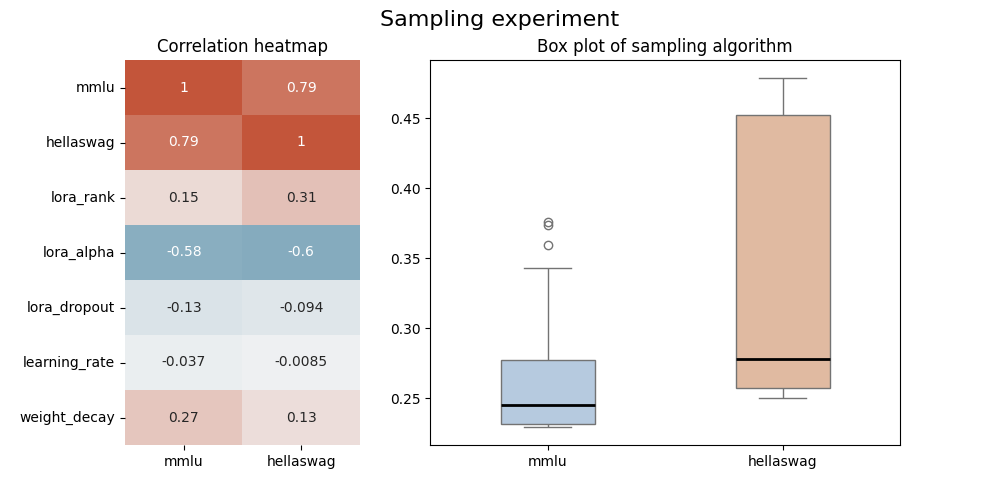
\includegraphics[width=0.6\linewidth]{figures/sampling/lhs.png}
    \caption{Results of \acrlong{lhs} experiment}
    \label{fig:lhs_exp}
\end{figure}

The correlation between MMLU and Hellswag tend to confirm the relevance of their choice as a pair for validation and testing dataset. It's sufficiently high to guess that most of the \textit{good} solution for one will be good for the other one, but it's still less than one, making over-fitting visible if present.

For variables, it looks like LoRA alpha, the scaling parameter of LoRA, is the most influent on the score, be it Hellaswag or MMLU. Next to it, LoRA Rank and weight decay are the most influent, with a difference in ranking on the metrics. With this first exploration, it looks like Dropout and Learning rate are not very effectful for this problem, be it the choice of their range or the implementation. 

On the distribution of the score values, it's interesting to note that Hellaswag has a broader range of score, making it useful for efficiently discriminating solutions.  With a broader thinking, the sampling experiment confirm the relevance to apply \acrshort{hpo} algorithms to the described problem. If scores were independent of variables, or all scores were the same, \acrshort{hpo} would be useless. 

%%%%%%%%%%%%%%%%%%%% BO Experiment %%%%%%%%%%%%%%%%%%%%%%%%%%
\subsection{\acrshort{bogp} experiment}
\label{sec:bo_exp}
Figure \ref{fig:bo_res} depicts the performance of \acrfull{bogp} over 50 iterations, measured in terms of the \Gls{hs} accuracy. This visualization highlights the evolution of the optimization process as it transitions from sampling to the exploitation, and ultimately converges towards high-performing solutions.


\begin{figure}[h!]
    \centering
    \begin{subfigure}[b]{.50\textwidth}
      \centering
      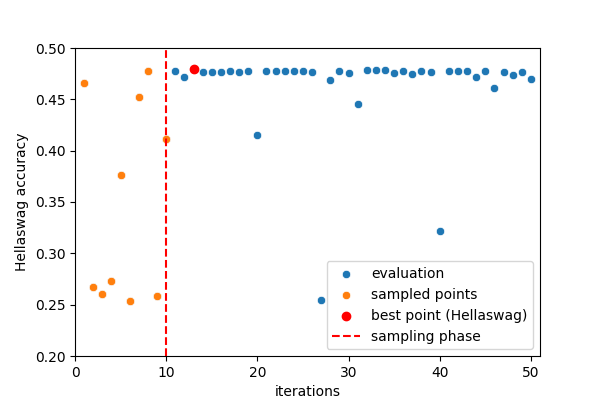
\includegraphics[width = \textwidth]{figures/bo/score_evolution.png}
      \caption{Score over time}
      \label{fig:bo_score_time}
    \end{subfigure}%
    \begin{subfigure}[b]{.40\textwidth}
      \centering
      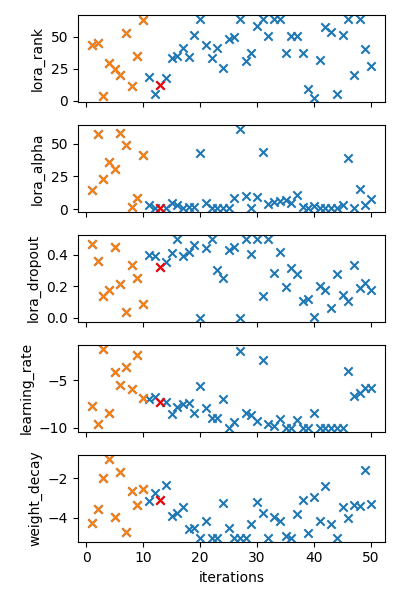
\includegraphics[width = 0.6\textwidth]{figures/bo/variables_evolution.png}
      \caption{Variable over time}
      \label{fig:bo_var_time}
    \end{subfigure}
    \caption{Experiment using \acrshort{bo} algorithm}
    \label{fig:bo_res}
\end{figure}

During the sampling phase, as shown by figure \ref{fig:bo_score_time}, evaluated solutions have the same diversity of solutions than the full sampling experiment, allowing to efficiently extract knowledge from the search space. The algorithm achieves a stable convergence to mostly high-performing solution.

If we briefly look at figure \ref{fig:bo_var_time}, it's interesting to look at the diversity of configuration to obtain high-performance, and the trend of the algorithms for each variable. For instance, for LoRA alpha, or learning rate, we can observe a clear trend toward the lower bound of the optimization range. 

To summarize, this experiment demonstrate the effectiveness of Bayesian Optimization in efficiently exploiting the knowledge of the search space obtained in the sampling phase. The optimization process still explores area with high uncertainty, giving few low-performing solution.


%%%%%%%%%%%%%%%%%%%% SOO Experiment %%%%%%%%%%%%%%%%%%%%%%%%%%
\subsection{\acrshort{soo} experiment}
\label{sec:soo_exp}

On this experiment, we observe in Figure \ref{fig:soo_res} the behavior of \acrshort{soo} as it optimizes the given objective function. The figure illustrates how the algorithm navigates the search space, iteratively improving the solution by adjusting the hyperparameters. By examining the trends in performance metrics and variables evolution, we aim to analyze the convergence behavior, stability, and overall effectiveness of \acrshort{soo} in this setting.

\begin{figure}[h!]
    \centering
    \begin{subfigure}[b]{.5\textwidth}
      \centering
      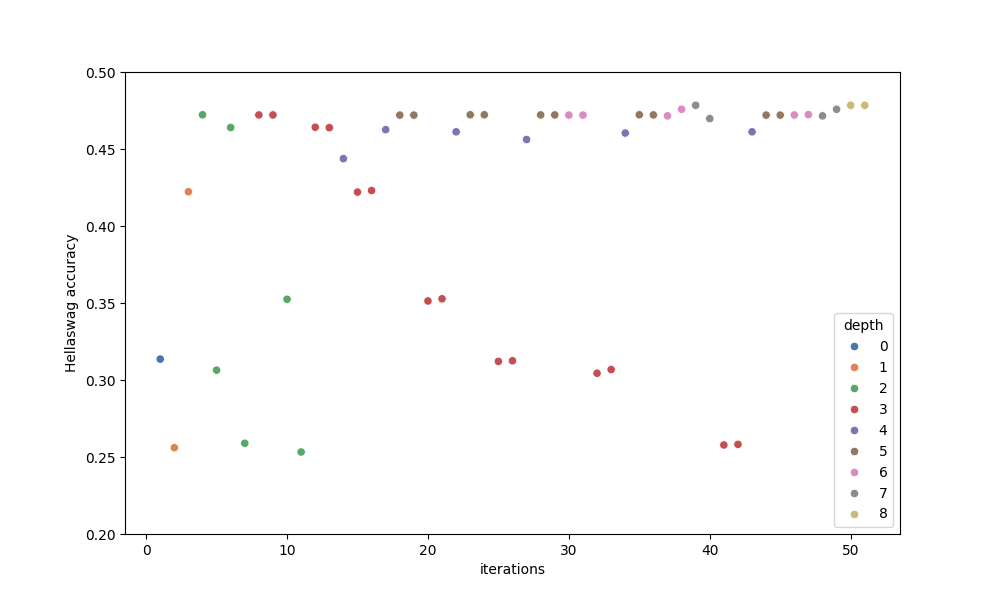
\includegraphics[width = \textwidth]{figures/soo/score_evolution.png}
      \caption{Score over time}
      \label{fig:soo_score_time}
    \end{subfigure}%
    \begin{subfigure}[b]{.4\textwidth}
      \centering
      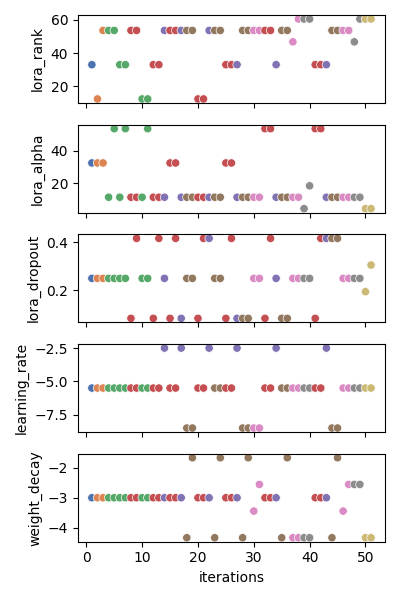
\includegraphics[width = 0.5\textwidth]{figures/soo/variables_evolution.png}
      \caption{Variable values over time}
      \label{fig:soo_var_time}
    \end{subfigure}
    \caption{Experiment using \acrshort{soo} algorithm}
    \label{fig:soo_res}
\end{figure}


Figure \ref{fig:soo_score_time} depicts the accuracy of the \gls{hs} dataset as a function of iterations, with marker colors representing different depth configurations. The observed trend suggests that most configurations achieve accuracies around 0.46 throughout the optimization process. Several configurations converge toward the higher end of this range, indicating potential stability and effectiveness in learning as iterations progress. 

It is evident that higher-depth configurations tend to cluster around higher accuracy values, while lower depths display more scattered behavior across the accuracy spectrum. In specific, depth 2, with a section on lora alpha seems to greatly affect the performance on the accuracy. On figure \ref{fig:soo_var_time}, it's clear on the limitation of constrained-budget \acrshort{soo} without local exploitation at the end of the algorithms : Only a few number of values by variables are explored : around 5 by variables, making it equivalent to exploration of a search space of $6^5=7,776$ discrete solutions.

To summarize, \acrshort{soo} achieve a maximum performance closed to the precedent algorithm, but explore a restricted number of configuration, and lose time by evaluating unpromising solutions.
%%%%%%%%%%%%%%%%%%%% BaMSOO Experiment %%%%%%%%%%%%%%%%%%%%%%%%%%
\subsection{\acrshort{bamsoo} experiment}
\label{sec:bamsoo_exp}

The last experiment of this work is using \acrshort{bamsoo}, with $\eta = 1$ in equation \ref{eq:ucb}, to reduce the confidence interval and promote approximation, to avoid the evaluation of unpromising points. To look after it, figure \ref{fig:bamsoo_score_time} discriminate evaluated and approximated points, and might be compared with \ref{fig:soo_score_time} to look after approximated points.



\begin{figure}[h]
    \centering
    \begin{subfigure}[b]{.5\textwidth}
      \centering
      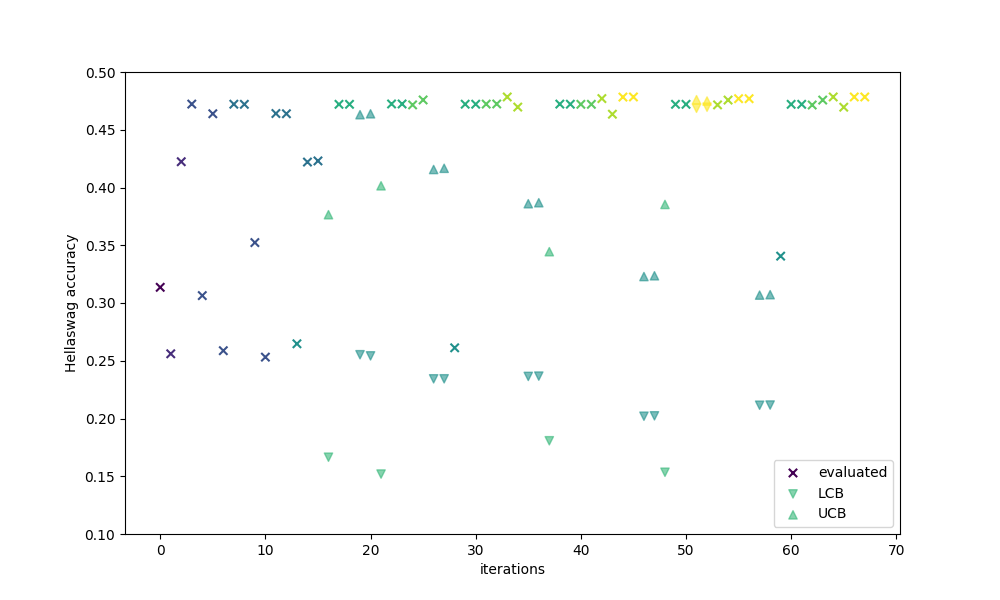
\includegraphics[width = 0.9\textwidth]{figures/bamsoo/score_evolution.png} 
      \caption{Score over time}
      \label{fig:bamsoo_score_time}
    \end{subfigure}%
    \begin{subfigure}[b]{.4\textwidth}
      \centering
      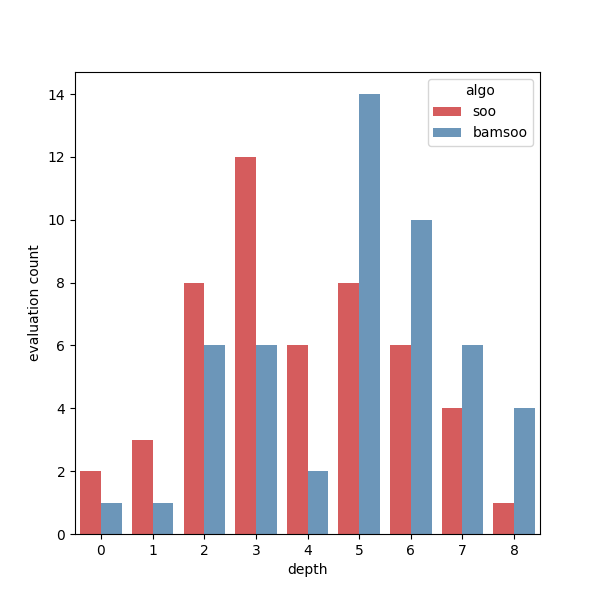
\includegraphics[width = 0.7\textwidth]{figures/bamsoo/depth_compar.png} 
      \caption{Depth exploration }
      \label{fig:bamsoo_soo_depth}
    \end{subfigure}
    \caption{Experiment using \acrshort{bamsoo} algorithm}
    \label{fig:bamsoo_res}
\end{figure}

When compared to figure \ref{fig:soo_score_time}, the pair of evaluations for depth 2, with low-performing solutions seems to have mostly been approximated. On the whole experiment, 16 points were approximated, to efficiently search further than \acrshort{soo}. Figure \ref{fig:bamsoo_soo_depth} compare the budget allowed on each depth, and highlight the focus of \acrshort{bamsoo} for lower depth exploration.
To summarize, \acrshort{bamsoo} achieve to speed up \acrshort{soo}, but is still slow in comparison with \acrshort{bo} at first glance. Moreover, \acrshort{bamsoo} succeed to prevent most of low-performing evaluation of \acrshort{soo}.








%%%%%%%%%%%%%%%%%%%% Analysis %%%%%%%%%%%%%%%%%%%%%%%%%%

\subsection{Comparison and Analysis}
\label{sec:comparison}

To conclude this section, it's crucial to directly compare algorithms, especially their performance, with validation and testing dataset. To look at absolute performance, and not only relative between algorithms, lower and upper bounds will be used. 

\begin{table}[h!]
    \centering
    \begin{tabular}{|c||c|c||c|c|c|}
    \hline
       Datasets  & Lower (LHS) & Upper (model card) & BO-GP & SOO & BaMSOO \\
    \hline
       Hellaswag (validation)  & 47.90 & 41.5 & 47.91 & 47.84 & 47.84\\
       MMLU (testing) & 37.61 & 49.3 & 38.11 & 37.42 & 37.50 \\
    \hline
    \end{tabular}
    \caption{Bounds on accuracy for validation and testing dataset}
    \label{tab:bounds}
\end{table}
In face of such experiments, it's interesting to look at bounds of the metric, to compare the results. The lower bounds are the results of the experiment using solely \acrshort{lhs} to pick solutions, with the same number of evaluation than algorithms. \acrshort{lhs} being intrinsically parallel, if evaluated algorithms don't achieve better performance than a solely exploring one, their benefit isn't relevant. 

For the higher bound, I will look at the higher value in the model card\footnote{\url{https://huggingface.co/meta-llama/Llama-3.2-1B}} of the model, achieved using advanced fine-tuning methods like Supervised Fine-Tuning (SFT), Rejection Sampling (RS), and Direct Preference Optimization (DPO). Values are inside table \ref{tab:bounds}.

\begin{figure}[h]
    \centering
    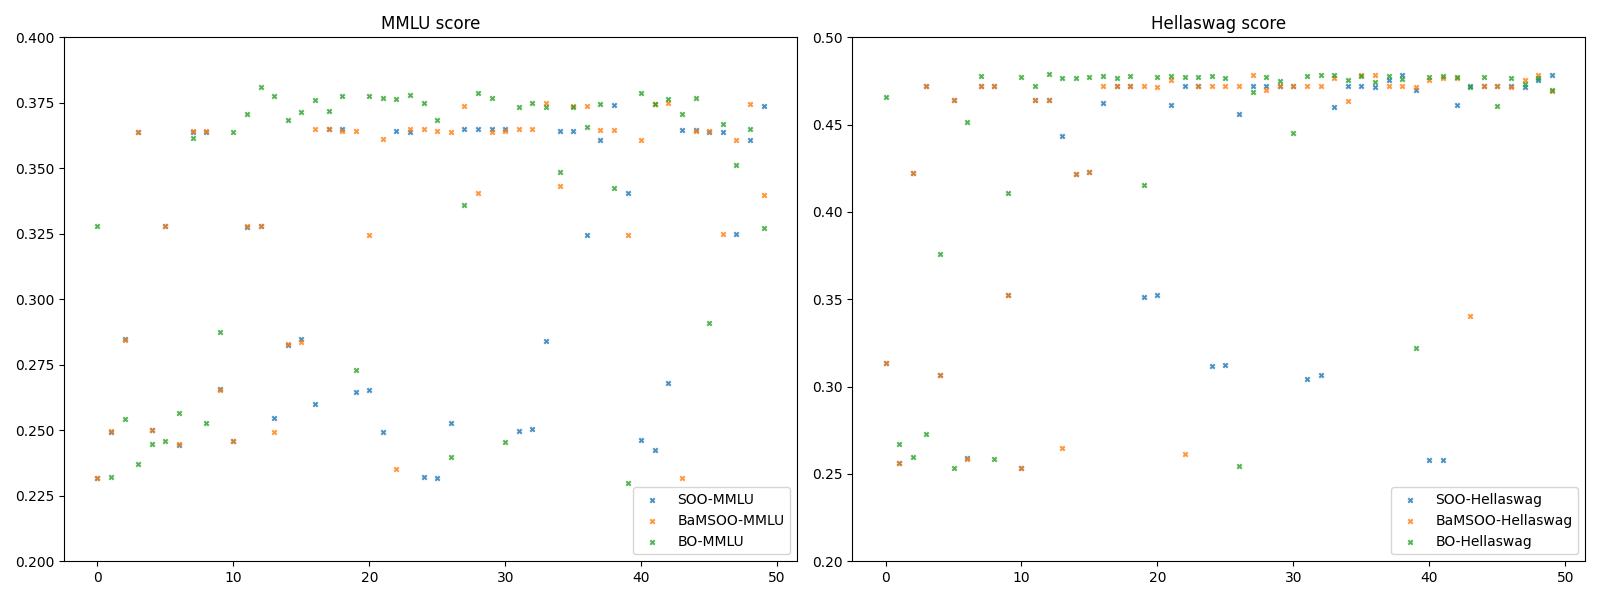
\includegraphics[width=0.8\textwidth]{figures/global/comparison.png}
    \caption{Comparison between 3 algorithms on 2 metrics}
    \label{fig:global_compare}
\end{figure}


At first, what's interesting is to look at testing and upper bounds results. Since the upper bound is mostly fine-tuned with aimed for MMLU results, the \Gls{hs} upper bounds isn't really relevant. Considering this, the analysis of this part will mostly be done with MMLU. The best results with MMLU is \acrfull{bo}, being 23\% from the upper bound.




With figure \ref{fig:global_compare}, it's clearer than \acrshort{bo} algorithm is a step more performing than others algorithms for this problem, especially with the low number of low-performing solutions evaluated. Apart from this part, the whole results may suggest that the objective function, or the search space could be different, to have an higher range of results for comparison. 











\section{Conclusions and Perspectives}
\label{sec:conclusion}

For scenarios with a limited number of evaluations, \acrshort{bo} demonstrated exceptional efficiency, quickly converging to high-performing solutions. In contrast, \acrshort{soo}, constrained by one-dimensional sections and less promising search dynamics, exhibited slower convergence. The hybrid approach, \acrshort{bamsoo}, successfully enhanced the convergence rate of \acrshort{soo} while preserving its inherent parallelism capabilities.

This work pioneers the application of hybrid Bayesian and partition-based optimization for expensive functions, laying the groundwork for scaling the efficiency of Bayesian Optimization to exascale computing environments.

Future research should explore higher-performance architectures, larger models, and expanded datasets to effectively distribute the computational load across supercomputers. Additionally, extending the search space to include hyperparameters such as Adam momentum would provide new opportunities to further refine optimization strategies.
  




%End of the paper (acknowledgment, biblio, biography...) 
%\clearpage

\section*{Acknowledgments}
This work was partially supported by the EXAMA (Methods and Algorithms at Exascale) project under grant ANR-22-EXNU-0002.


Experiments presented in this paper were carried out using the Grid'5000 testbed, supported by a scientific interest group hosted by Inria and including CNRS, RENATER and several Universities as well as other organizations (see https://www.grid5000.fr).

\bibliographystyle{splncs}
\bibliography{latex_files/HPO}


\end{document}
